\documentclass[tikz,border=6pt]{standalone}
\usepackage{amsmath,amssymb}
\begin{document}
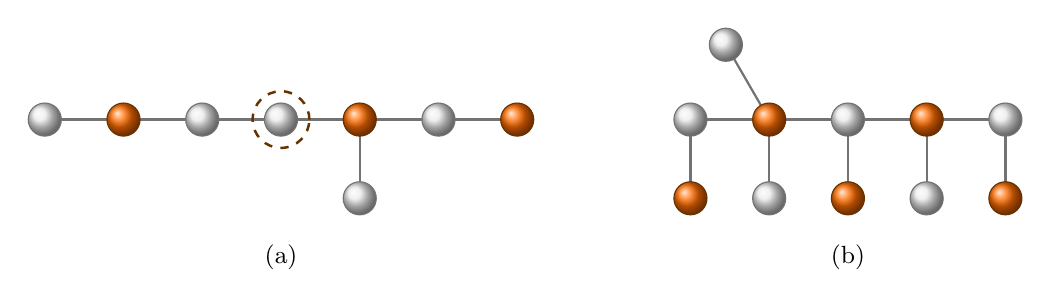
\begin{tikzpicture}[x=1.0cm,y=1cm,
  v/.style={circle,shading=ball,ball color=white!92!black,draw=black!55,minimum size=4.2mm,inner sep=0pt},
  d/.style={v,ball color=orange!85!red,draw=orange!40!black},
  e/.style={draw=black!55,line width=0.8pt},
  lab/.style={font=\footnotesize,inner sep=1pt}]
  % (a) the 8-vertex tree: path a1..a7, pendant at a5; centre a4; an independent dominating set of size 3
  \begin{scope}
    \foreach \k in {1,...,7} \coordinate (a\k) at (\k-1,0);
    \coordinate (a8) at (4,-1.0);
    \draw[e] (a1)--(a2)--(a3)--(a4)--(a5)--(a6)--(a7); \draw[e] (a5)--(a8);
    \draw[orange!40!black,line width=0.9pt,dashed] (a4) circle (3.6mm);
    \foreach \k in {1,3,4,6,8} \node[v] at (a\k) {};
    \foreach \k in {2,5,7} \node[d] at (a\k) {};
    \node[font=\small] at (3,-1.75) {(a)};
  \end{scope}
  % (b) F_5: path b1..b5, a pendant at each, a second pendant at b2; an independent dominating set of size 5
  \begin{scope}[xshift=8.2cm]
    \foreach \k in {1,...,5} { \coordinate (b\k) at (\k-1,0); \coordinate (l\k) at (\k-1,-1.0); }
    \coordinate (l6) at (0.45,0.95);
    \draw[e] (b1)--(b2)--(b3)--(b4)--(b5);
    \foreach \k in {1,...,5} \draw[e] (b\k)--(l\k);
    \draw[e] (b2)--(l6);
    \foreach \k in {1,3,5} \node[v] at (b\k) {};
    \foreach \k in {2,4,6} \node[v] at (l\k) {};
    \foreach \k in {2,4} \node[d] at (b\k) {};
    \foreach \k in {1,3,5} \node[d] at (l\k) {};
    \node[font=\small] at (2,-1.75) {(b)};
  \end{scope}
\end{tikzpicture}
\end{document}
